
\begin{tikzpicture}[node distance=2cm, auto]
    % Nodes
    \node [draw, rectangle, minimum width=2cm, minimum height=1cm, align=center, label=above:$x(t)$, label=below:Stimulus] (stimulus) {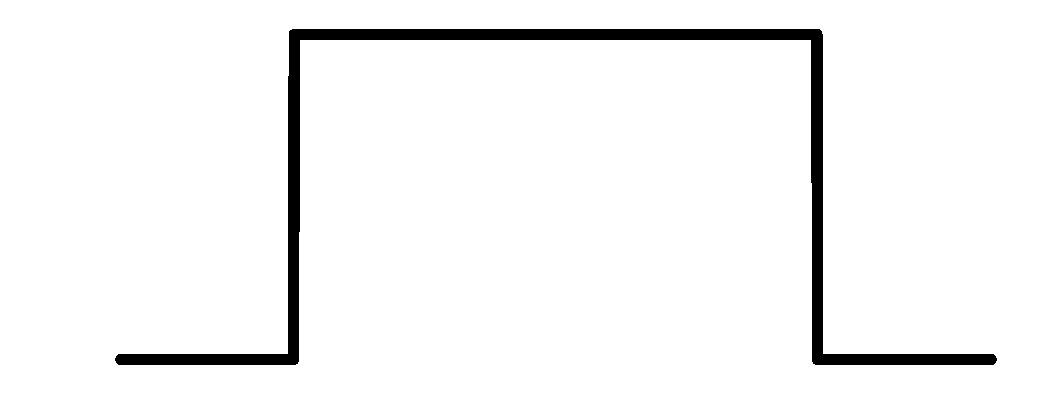
\includegraphics[scale=0.15]{IMAGES/BACKGROUND/stim.pdf}};
    
    \node [draw, fill=blue!20, rectangle,  minimum width=11.6cm, minimum height=8cm, right=0.5cm of stimulus,  label=above:\textbf{GLM}, , shift={(0, -1.3)} ] (GLM_Box) {};

    \node [draw, fill=white, rectangle,  minimum width=2.5cm, minimum height=2.5cm, right=1cm of stimulus, align=center, label=above:$k$, label={[align=center]below:Feedforward \\ filter}] (k) {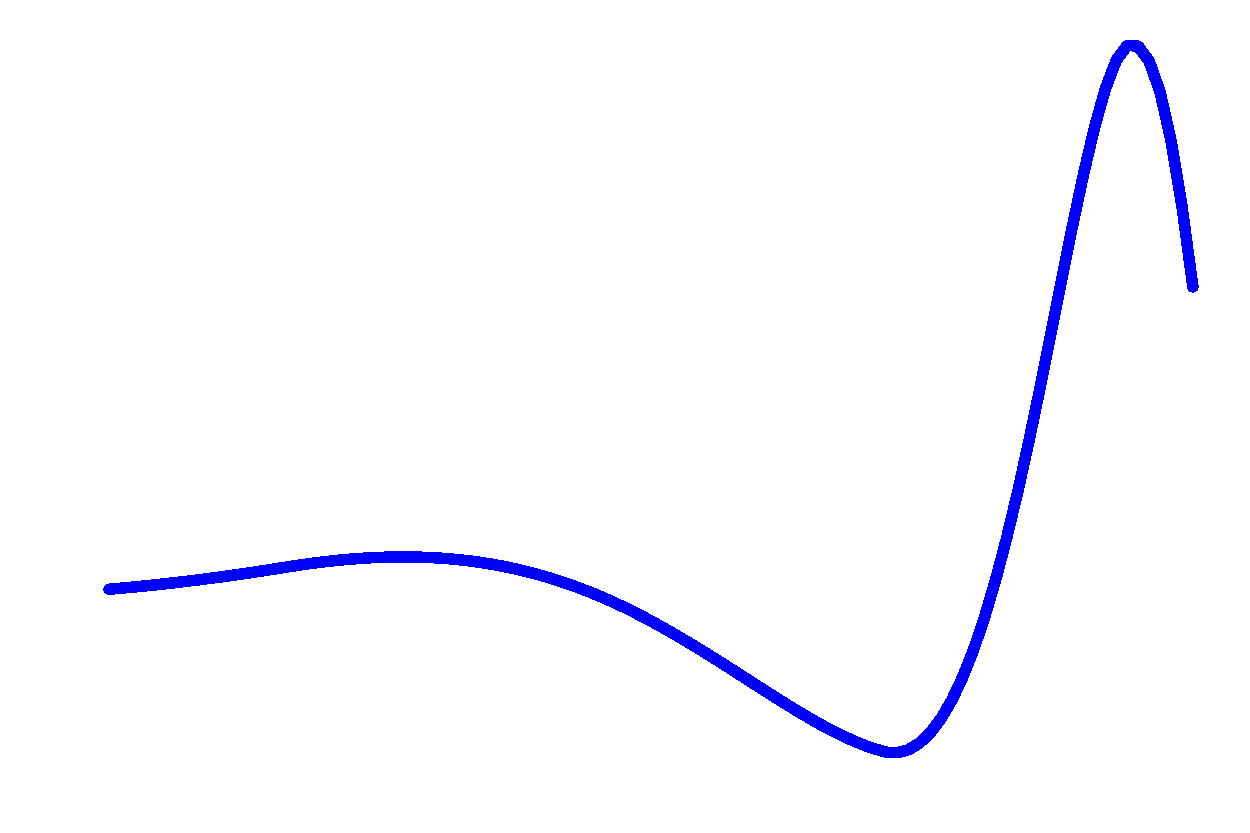
\includegraphics[scale=0.1]{IMAGES/BACKGROUND/kfilter.pdf}};

    \node [draw, fill=white, circle, right=0.5cm of k, align=center] (plus) {+};

    \node [draw, fill=white, rectangle, minimum width=1cm, minimum height=1cm, above=0.5cm of plus, align=center ,label={[align=center]above:Constant}] (cst) {C};
    
    \node [draw, fill=white, rectangle,  minimum width=2.5cm, minimum height=2.5cm, right=0.5cm of plus, align=center, label=above:$f$, label={[align=center]below:Nonlinear \\ function}] (f) {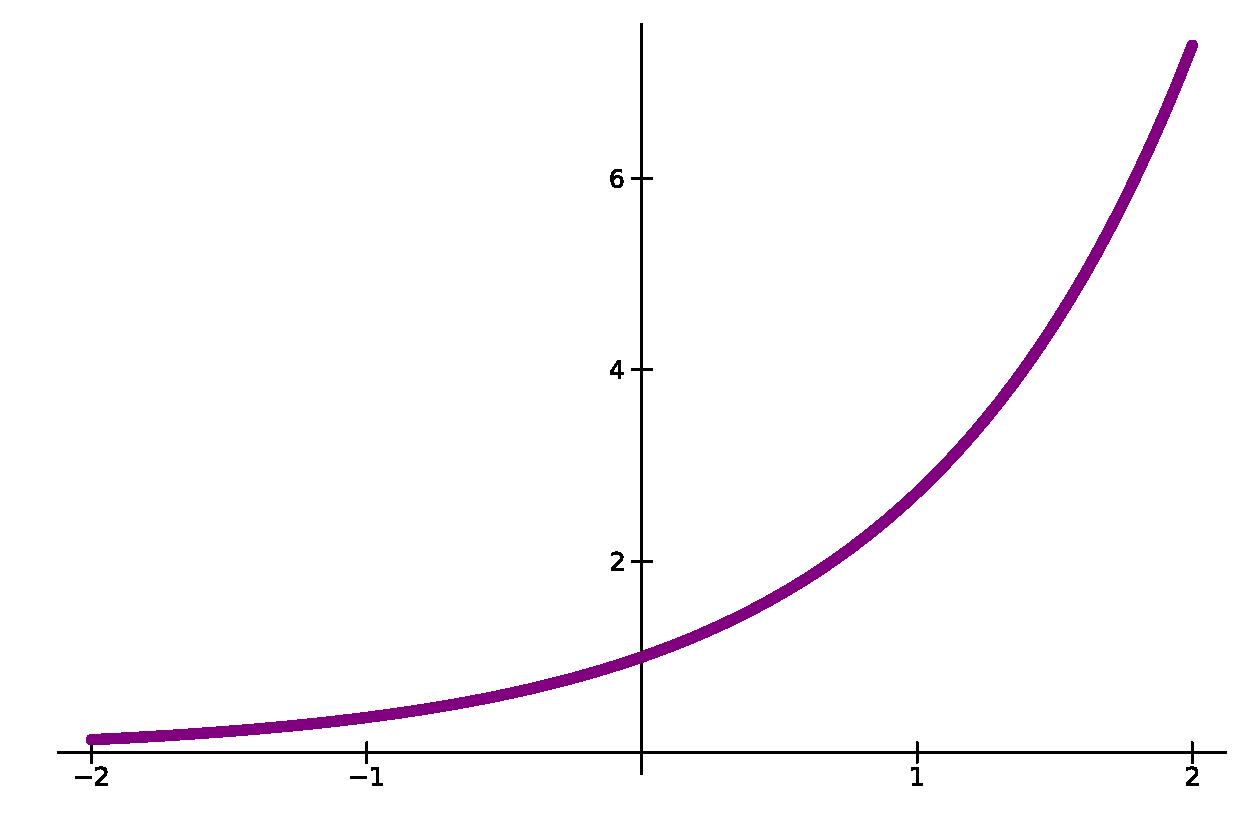
\includegraphics[scale=0.1]{IMAGES/BACKGROUND/ffunction.pdf}};

    \node [draw, fill=white, rectangle,  minimum width=2.5cm, minimum height=2.5cm, right=1cm of f, align=center, label=above:, label={[align=center]below:Stochastic \\ process}] (Aleatoire) {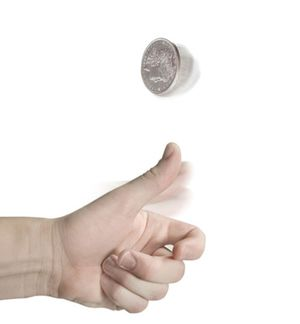
\includegraphics[scale=0.2]{IMAGES/BACKGROUND/Stocha_process.jpg}};

    \node [draw, rectangle,  minimum width=2cm, minimum height=1cm, right=1cm of Aleatoire, align=center, label=above:$y(t)$, label=below:Responses ] (y) {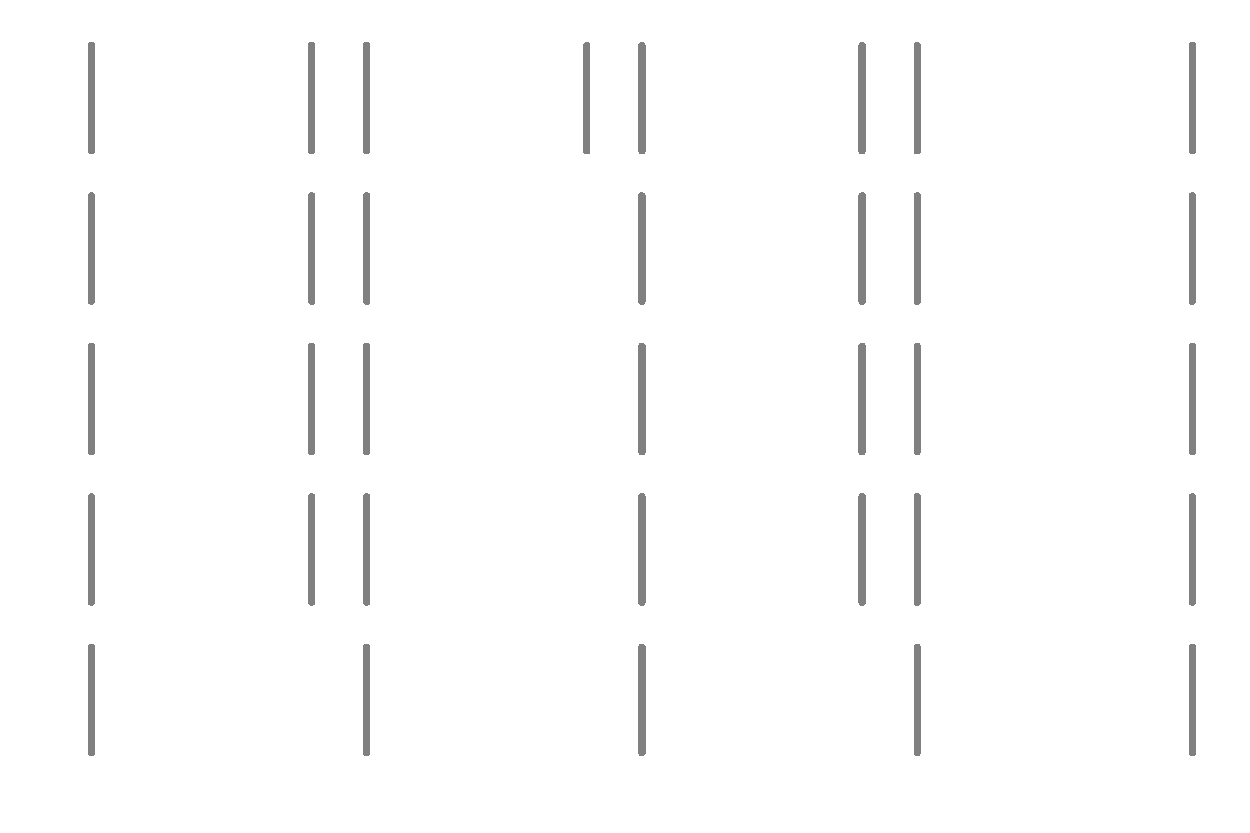
\includegraphics[scale=0.1]{IMAGES/BACKGROUND/y_out.pdf}};

    \node [draw, fill=white, rectangle,  minimum width=2cm, minimum height=1cm, above=-5.5cm of f, align=center, label=above:$h$, label={[align=center]below:Feedback \\ filter},  shift={(1.5, 0)} ] (h) {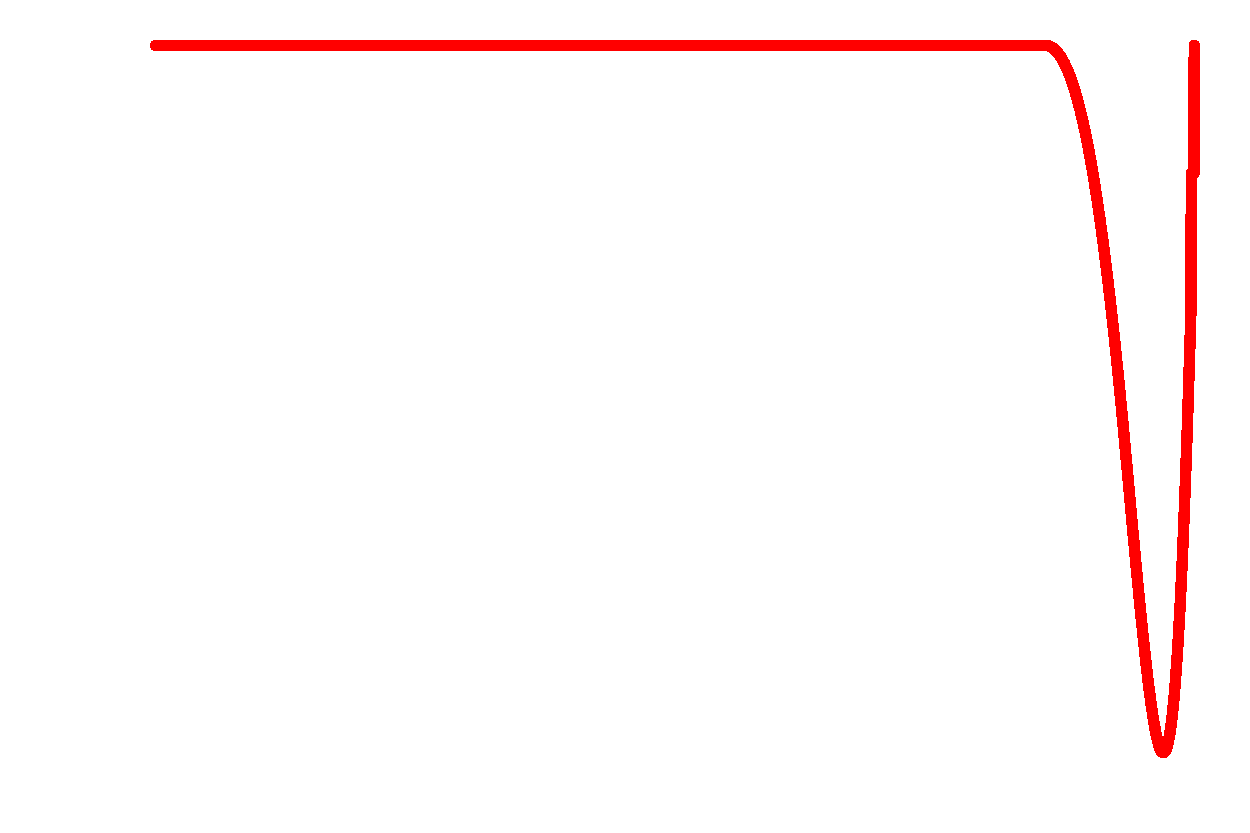
\includegraphics[scale=0.1]{IMAGES/BACKGROUND/hfilter.pdf}};


    

    % Arrows
    \draw [->] (stimulus) -- (k);
    \draw [->] (k) -- (plus);
    \draw [->] (cst) -- (plus);
    \draw [->] (plus) -- (f);
    \draw [->] (f) -- node[above] {$\lambda (t)$} (Aleatoire);
    \draw [->] (Aleatoire) -- (y);

\draw (Aleatoire.east) edge[->, out=0, in=0,] (h.east);
 %\draw [arrow] (Aleatoire) to [bend left=20] (h);

\draw  (h.west) edge[->, out=180, in=270] (plus.south);


  
\end{tikzpicture}